% !TEX root = ../main.tex
\section{针对存在故障情况的模型检验}
	\subsection{模型的假设与标记}
		\subsubsection{假设}
			\begin{enumerate}
				\item\label{故障发生概率}所有CNC故障的发生服从独立且参数相同的两点分布;
				\item\label{故障发生时间}所有CNC故障的发生时间服从独立且参数相同的均匀分布,发生时间的取值区间下界为加工开始时间,上界为加工结束时间。
			\end{enumerate}
		\subsubsection{标记}
			\begin{table}[htbp]
				\centering
				\caption{标记:针对存在故障情况的模型检验}
				\label{标记:针对存在故障情况的模型检验}
				\begin{longtabu}to\linewidth{@{}X[c]|X[l]@{}}
					\toprule
					变量&定义\\\midrule
					\(T_\mathrm{machine}\)&CNC加工时间\\
					\(t_\mathrm{repair}\)&CNC修理时间\\
					\(t_\mathrm{machineMax}\)&不发生故障时的CNC加工时间\\\bottomrule
				\end{longtabu}
			\end{table}
	\subsection{模型的建立与求解}
		\subsubsection{建立}
			模拟故障发生:随机生成一个在1到100之间的随机整数,若该数等于1,则认为发生故障。
			模拟故障发生时间:随机生成一个在0到1之间的随机数,该数乘以加工时间即为故障发生时间。
			\begin{figure}[htbp]
				\centering
				\caption{发生故障的机器周期}
				\label{发生故障的机器周期}
				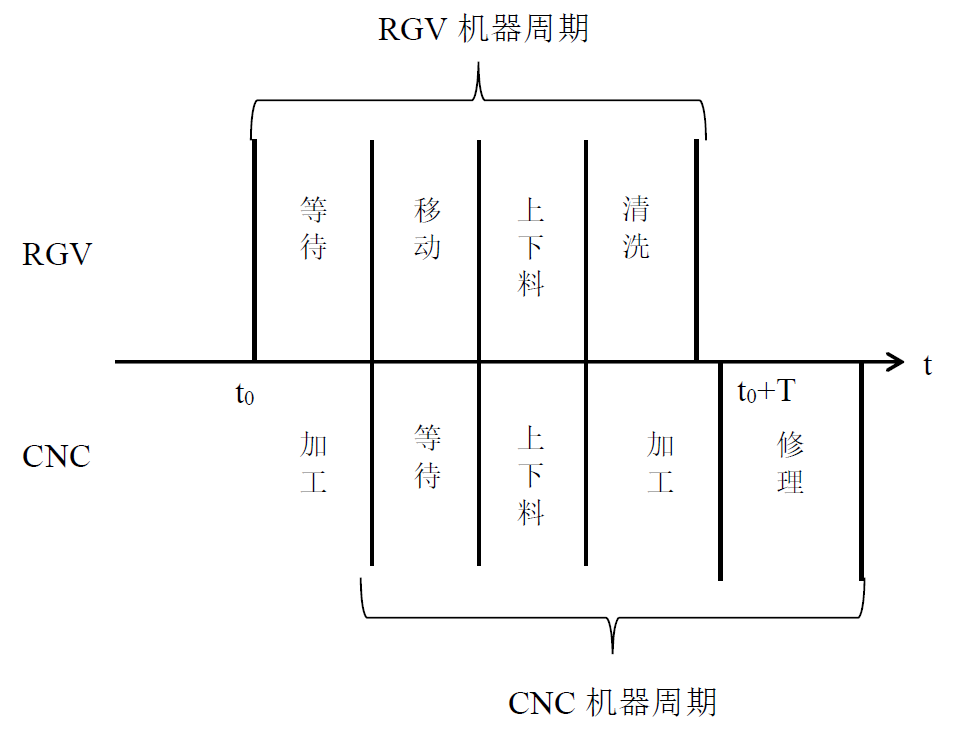
\includegraphics[width=10cm]{graph/periodFault.png}
			\end{figure}
			\par\indent 若CNC发生故障,损耗时间包括已加工时间以及额外的修理时间,如图\ref{发生故障的机器周期}和公式\ref{发生故障的机器周期公式}。
			\begin{align}
				\label{发生故障的机器周期公式}
				T_\mathrm{CNC}=T_\mathrm{wait}+T_\mathrm{update}+T_\mathrm{machine}+T_{repair} \\
				0\leqslant T_\mathrm{machine}\leqslant T_\mathrm{machineMax}
			\end{align}
			\par\indent 发生故障会导致该轮循环熟料总数不变,且该CNC恢复到初始无料状态。
			\begin{figure}[htbp]
				\centering
				\caption{程序流程图:针对存在故障情况的模型检验}
				\label{程序流程图:针对存在故障情况的模型检验}
				\begin{tikzpicture}[align = center, node distance = 1.5cm]
					\node(开始)[startstop]{开始};
					\node(循环开始)
					[	process,
						below of = 开始
					]{循环开始};
					\node(是否有CNC发出信号?)
					[	decision,
						below of = 循环开始,
						yshift = -.5cm
					]{是否\\有CNC发出\\信号?};
					\node(等待)
					[	process,
						right of = 是否有CNC发出信号?,
						xshift = 3cm,
						yshift = 2cm
					]{等待};
					\node(有多个CNC发出信号;调用调度算法计算将被服务的CNC)
					[	io,
						below of = 是否有CNC发出信号?,
						yshift = -.5cm
					]{有多个CNC发出信号;\\调用调度算法计算将被服务的CNC};
					\node(RGV移动,CNC就绪)
					[	process,
						below of = 有多个CNC发出信号;调用调度算法计算将被服务的CNC
					]{RGV移动,CNC就绪};
					\node(RGV上下料,CNC上下料)
					[	process,
						below of = RGV移动,CNC就绪
					]{RGV上下料,CNC上下料};
					\node(CNC是否故障?)
					[	decision,
						below of = RGV上下料,CNC上下料
					]{CNC是否故障?};
					\node(随机生成CNC故障时间;RGV清洗,CNC故障,CNC修理)
					[	process,
						right of = CNC是否故障?,
						xshift=4.5cm,
						yshift=-1.5cm
					]{随机生成CNC故障时间;\\RGV清洗,CNC故障,CNC修理};
					\node(下回无需清洗,无法输出熟料,CNC增加1个机器周期)
					[	io,
						below of = 随机生成CNC故障时间;RGV清洗,CNC故障,CNC修理
					]{下回无需清洗,无法输出熟料,\\CNC增加1个机器周期};
					\node(RGV清洗,CNC加工)
					[	process,
						below of = CNC是否故障?
					]{RGV清洗,CNC加工};
					\node(成品数加1,CNC增加1个机器周期)
					[	io,
						below of = RGV清洗,CNC加工
					]{成品数加1,\\CNC增加1个机器周期};
					\node(是否超时?)
					[	decision,
						below of = 成品数加1,CNC增加1个机器周期
					]{是否超时?};
					\node(时间增加1个RGV机器周期,刷新CNC冷却时间)
					[	process,
						left of = 循环开始,
						xshift = -3cm
					]{时间增加1个RGV机器周期,\\刷新CNC冷却时间};
					\node(结束)
					[	startstop,
						below of = 是否超时?
					]{结束};
					\draw[arrow](开始)--(循环开始);
					\draw[arrow](循环开始)--(是否有CNC发出信号?);
					\draw[arrow](是否有CNC发出信号?)-|node[right]{否}(等待);
					\draw[arrow](等待)--(循环开始);
					\draw[arrow](是否有CNC发出信号?)--node[right]{是}(有多个CNC发出信号;调用调度算法计算将被服务的CNC);
					\draw[arrow](有多个CNC发出信号;调用调度算法计算将被服务的CNC)--(RGV移动,CNC就绪);
					\draw[arrow](RGV移动,CNC就绪)--(RGV上下料,CNC上下料);
					\draw[arrow](RGV上下料,CNC上下料)--(CNC是否故障?);
					\draw[arrow](CNC是否故障?)-|node[right]{是}(随机生成CNC故障时间;RGV清洗,CNC故障,CNC修理);
					\draw[arrow](随机生成CNC故障时间;RGV清洗,CNC故障,CNC修理)--(下回无需清洗,无法输出熟料,CNC增加1个机器周期);
					\draw[arrow](下回无需清洗,无法输出熟料,CNC增加1个机器周期)|-(是否超时?);
					\draw[arrow](CNC是否故障?)--node[right]{否}(RGV清洗,CNC加工);
					\draw[arrow](RGV清洗,CNC加工)--(成品数加1,CNC增加1个机器周期);
					\draw[arrow](成品数加1,CNC增加1个机器周期)--(是否超时?);
					\draw[arrow](是否超时?)-|node[left]{否}(时间增加1个RGV机器周期,刷新CNC冷却时间);
					\draw[arrow](时间增加1个RGV机器周期,刷新CNC冷却时间)--(循环开始);
					\draw[arrow](是否超时?)--node[right]{是}(结束);
				\end{tikzpicture}
			\end{figure}
			\par\indent 程序流程如图\ref{程序流程图:针对非抢占式排队系统的静态调度模型}。
		\subsubsection{求解}
			程序清单\ref{主程序}和\ref{模拟退火搜索最优静态调度和最优CNC工序分配分布的主程序}给出了故障率输入的参数。运行结果\ref{主程序结果}就是一个存在故障情况的运行结果。
